\chapter{Classification}
\section{Introduction}

In statistical classification, each object is represented by $d$ features (a
measurement vector), and the goal of classification becomes finding compact and
disjoint regions (decision regions\cite{Duda2000}) for classes in a
$d$-dimensional feature space. Such decision regions are defined by decision
rules that are known or can be trained.  The simplest configuration of a
classification consists of a decision rule and multiple membership functions;
each membership function represents a class. Figure~\ref{fig:simple}
illustrates this general framework.

\begin{figure}[h]
  \centering
  \includegraphics[width=0.7\textwidth]{DudaClassifier.eps}
  \itkcaption[Simple conceptual classifier]{Simple conceptual classifier.}
  \label{fig:simple}
\end{figure}

This framework closely follows that of Duda and
Hart\cite{Duda2000}. The classification process can be described
as follows:

\begin{enumerate}
\item{A measurement vector is input to each membership function.}
\item{Membership functions feed the membership scores to the
    decision rule.}
\item{A decision rule compares the membership scores and returns a
    class label.}
\end{enumerate}

\begin{figure}
  \centering
  \includegraphics[width=0.7\textwidth]{StatisticalClassificationFramework.eps}
  \itkcaption[Statistical classification framework]{Statistical classification
framework.}
  \protect\label{fig:StatisticalClassificationFramework}
\end{figure}

This simple configuration can be used to formulated various classification
tasks by using different membership functions and incorporating task specific
requirements and prior knowledge into the decision rule. For example, instead
of using probability density functions as membership functions, through
distance functions and a minimum value decision rule (which assigns a class
from the distance function that returns the smallest value) users can achieve a
least squared error classifier. As another example, users can add a rejection
scheme to the decision rule so that even in a situation where the membership
scores suggest a ``winner'', a measurement vector can be flagged as ill
defined. Such a rejection scheme can avoid risks of assigning a class label
without a proper win margin.

\subsection{k-d Tree Based k-Means Clustering}
\label{sec:KdTreeBasedKMeansClustering}
\ifitkFullVersion
\input{KdTreeBasedKMeansClustering.tex}
\fi

\subsection{K-Means Classification}
\label{sec:KMeansClassifier}
\ifitkFullVersion
\input{ScalarImageKmeansClassifier.tex}
\fi
\ifitkFullVersion
\input{ScalarImageKmeansModelEstimator.tex}
\fi

\subsection{Bayesian Plug-In Classifier}
\label{sec:BayesianPluginClassifier}

\ifitkFullVersion 
\input{BayesianPluginClassifier.tex}
\fi


\subsection{Expectation Maximization Mixture Model Estimation}
\label{sec:ExpectationMaximizationMixtureModelEstimation}

\ifitkFullVersion 
\input{ExpectationMaximizationMixtureModelEstimator.tex}
\fi

\subsection{Classification using Markov Random Field}
\label{sec:MarkovRandomField}

Markov Random Fields are probabilistic models that use the correlation between
pixels in a neighborhood to decide the object region. The
\subdoxygen{itk}{Statistics}{MRFImageFilter} uses the maximum a posteriori (MAP)
estimates for modeling the MRF. The object traverses the data set and uses the
model generated by the Mahalanobis distance classifier to get the the distance
between each pixel in the data set to a set of known classes, updates the
distances by evaluating the influence of its neighboring pixels (based on a MRF
model) and finally, classifies each pixel to the class which has the minimum
distance to that pixel (taking the neighborhood influence under consideration).
The energy function minimization is done using the iterated conditional modes
(ICM) algorithm \cite{Besag1986}.

\ifitkFullVersion
\input{ScalarImageMarkovRandomField1.tex}
\fi 



\section{Support Vector Machines}
\label{sec:SupportVectorMachines}

Kernel based learning methods in general and the Support Vector
Machines (SVM) in particular, have been introduced in the last years
in learning theory for classification and regression tasks,
\cite{vapnik}. SVM have been successfully applied to text
categorization, \cite{joachims}, and face recognition,
\cite{osuna}. Recently, they have been successfully used for the
classification of hyperspectral remote-sensing images, \cite{bruzzoneSVM}.

Simply stated, the approach consists in searching for the separating
surface between 2 classes by the determination of the subset of
training samples which best describes the boundary between the 2
classes. These samples are called support vectors and completely
define the classification system. In the case where the two classes are
nonlinearly separable, the method uses a kernel expansion in order to make
projections of the feature space onto higher dimensionality spaces
where the separation of the classes becomes linear.

 \subsection{Mathematical formulation}

 This section reminds the basic principles of SVM learning and
 classification. A good tutorial on SVM can be found in, \cite{burges}.
 
We have $N$ samples represented by the couple $(y_i,\mathbf{x}_i),
i=1\ldots N$ where $y_i \in \{-1,+1\}$ is the class label and
$\mathbf{x}_i \in \mathbb{R}^n$ is the feature vector of dimension
$n$. A classifier is a function  $$f(\mathbf{x},\boldsymbol{\alpha}) :
\mathbf{x}\mapsto y$$ where $\boldsymbol{\alpha}$ are the classifier
parameters. The SVM finds the optimal separating hyperplane which
fulfills the following constraints :
    \begin{itemize}
      \item The samples with labels $+1$ and $-1$ are on different
      sides of the hyperplane.
      \item The distance of the closest vectors to the hyperplane is
      maximised. These are the support vectors (SV) and this distance is
      called the margin.
    \end{itemize}

    The separating hyperplane has the equation
    $$\mathbf{w}\cdot\mathbf{x}+b=0;$$ with $\mathbf{w}$ being its
    normal vector and $x$ being any point of the hyperplane. The
    orthogonal distance to the origin is given by
    $\frac{|b|}{\|\mathbf{w}\|}$. Vectors located outside the
    hyperplane have either $\mathbf{w}\cdot\mathbf{x}+b>0$ or
      $\mathbf{w}\cdot\mathbf{x}+b<0$.

    Therefore, the classifier function can be written as
    $$f(\mathbf{x},\mathbf{w}, b)=sgn(\mathbf{w}\cdot\mathbf{x}+b).$$
    
The SVs are placed on two hyperplanes which are parallel to the
      optimal separating one. In order to find the optimal
      hyperplane, one sets $\mathbf{w}$ and
      $b$ : $$\mathbf{w}\cdot\mathbf{x}+b=\pm 1.$$

Since there must not be any vector inside the margin, the following
constraint can be used:
    $$\mathbf{w}\cdot\mathbf{x}_i+b\ge +1\text{ if }y_i=+1;$$
    $$\mathbf{w}\cdot\mathbf{x}_i+b\le -1\text{ if }y_i=-1;$$ which
    can be rewritten as $$y_i(\mathbf{w}\cdot\mathbf{x}_i+b)-1\ge 0~  ~ \forall i.$$

    The orthogonal distances of the 2 parallel hyperplanes to the
    origin are $\frac{|1-b|}{\|\mathbf{w}\|}$ and
      $\frac{|-1-b|}{\|\mathbf{w}\|}$. Therefore the modulus of the
    margin is equal to $\frac{2}{\|\mathbf{w}\|}$ and it has to be
    maximised.

    Thus, the problem to be solved is:

	\begin{itemize}
	\item Find $\mathbf{w}$ and $b$ which minimise
	 $\left\{ \frac{1}{2}\|\mathbf{w}\|^2 \right\}$
	\item under the constraint :
	 $y_i(\mathbf{w}\cdot\mathbf{x}_i+b)\ge 1~  ~ i=1\ldots N.$
	\end{itemize}

	This problem can be solved by using the Lagrange multipliers
	with one multiplier per sample. It can be shown that only the
	support vectors will have a positive Lagrange multiplier.

	In the case where the two classes are not exactly linearly
	separable, one can modify the constraints above by using 
      $$\mathbf{w}\cdot\mathbf{x}_i+b\ge +1 - \xi_i \text{ if }y_i=+1;$$
    $$\mathbf{w}\cdot\mathbf{x}_i+b\le -1+\xi_i \text{ if }y_i=-1;$$
    $$\xi_i\ge 0~  ~\forall i.$$

	If $\xi_i > 1$, one considers that the sample is wrong. The
	function which has then to be minimised is
	$\frac{1}{2}\|\mathbf{w}\|^2 + C\left( \sum_i \xi_i\right); $,
	where $C$ is a tolerance parameter. The optimisation problem
	is the same than in the linear case, but one multiplier has to
	be added for each new constraint $\xi_i\ge 0$.

	If the decision surface needs to be non-linear, this solution
	cannot be applied and the kernel approach has to be adopted.


One drawback of the SVM is that, in their basic version, they can only
solve two-class problems. Some works exist in the field of multi-class
SVM (see \cite{allwein00reducing,weston98multiclass}, and the
comparison made by \cite{hsu01comparison}), but they are
not used in our system.

For problems with $N > 2$ classes, one can choose either to train $N$
SVM (one class against all the others), or to train $N\times(N-1)$ SVM
(one class against each of the others). In the second approach, which
is the one that we use, the final decision is taken by choosing the
class which is most often selected by the whole set of SVM.


\subsection{Learning With PointSets}
\label{sec:LearningWithPointSets}
\input{SVMPointSetModelEstimatorExample}
\subsection{PointSet Classification}
\label{sec:PointSetClassification}
\input{SVMPointSetClassificationExample}
\subsection{Learning With Images}
\label{sec:LearningWithImages}
\input{SVMImageModelEstimatorExample}
\subsection{Image Classification}
\label{sec:ImageClassification}
\input{SVMImageClassificationExample}
\input{SVMImageEstimatorClassificationMultiExample}

\section{Kohonen's Self Organizing Map}
\label{sec:SOM}
The Self Organizing Map, SOM, introduced by Kohonen is a
non-supervised neural
learning algorithm. The map is composed of neighboring cells which are
in competition by means of mutual interactions and they adapt in order
to match characteristic patterns of the examples given during the
learning. The SOM is usually on a plane (2D).

The algorithm implements a nonlinear projection from a high
dimensional feature space to a lower dimension space, usually 2D. It
is able to find the correspondence between a set of structured data
and a network of much lower dimension while keeping the topological
relationships existing in the feature space. Thanks to this
topological organization, the final map presents clusters and their
relationships. 

%\subsection{The algorithm}
Kohonen's SOM is usually represented as an array of cells where each
cell is, $i$, associated to a feature (or weight) vector  $\underline m_i = \left[m_{i1},m_{i2},\cdots,m_{in}\right]^T\in
\mathbb{R}^n$ (figure \ref{carte}).\\
\begin{figure}
\center
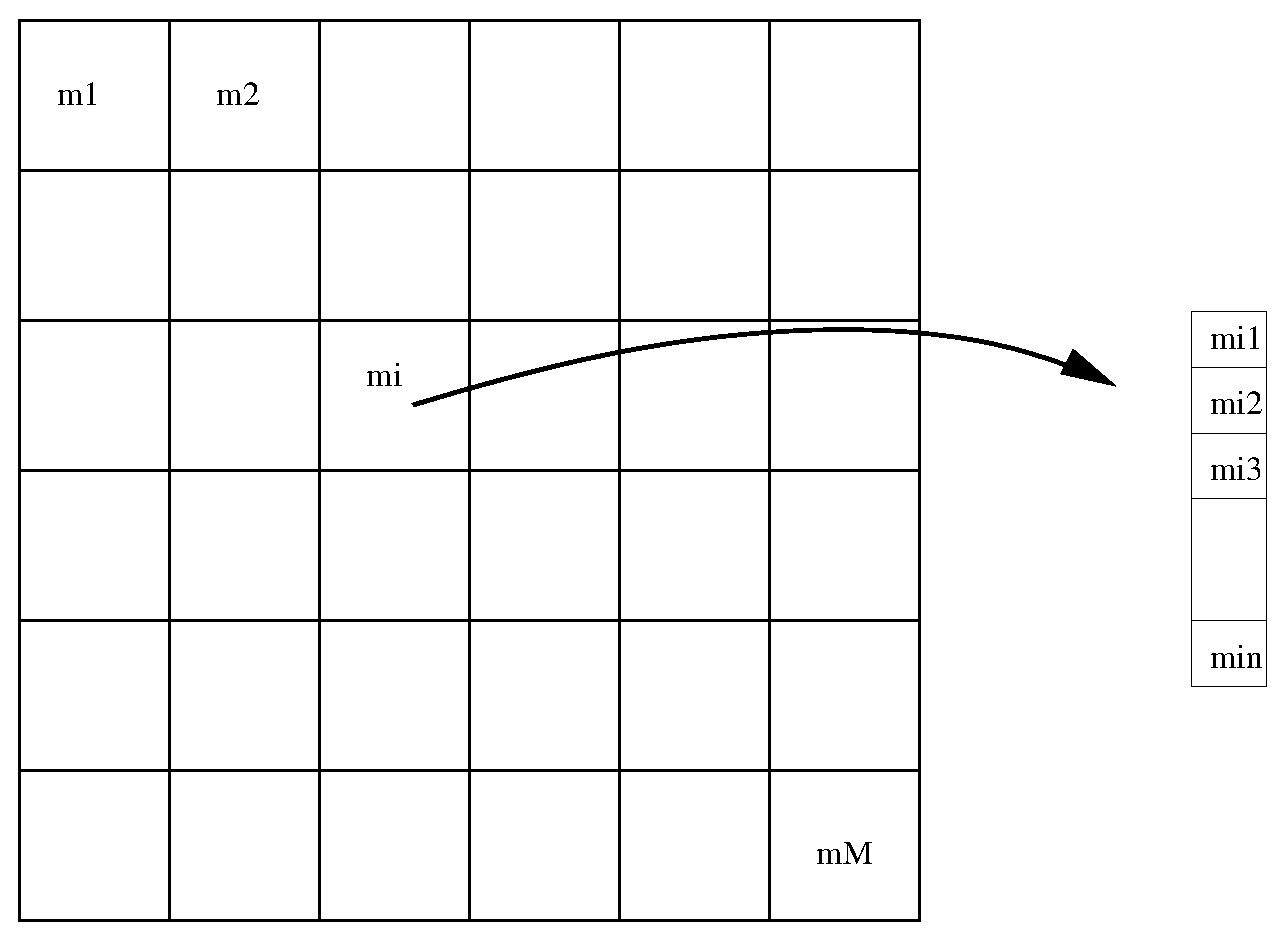
\includegraphics[width=0.45\textwidth]{carte.eps}
\itkcaption[Kohonen's Self Organizing Map]{Kohonen's Self Organizing Map}
\label{carte}
\end{figure}

A cell (or neuron) in the map is a good detector for a given input
vector $\underline x = \left[x_{1},x_{2},\cdots,x_{n}\right]^T\in
\mathbb{R}^n$ if the latter is {\em close} to the former. This
distance between vectors can be represented by the scalar product 
$\underline{x}^T\cdot\underline{m_i}$, but for most of the cases other
distances can be used, as for instance the Euclidean one. The cell
having the weight vector closest to the input vector is called the
{\em winner}.

%\subsubsection{Learning}
The goal of the learning step is to get a map which is representative
of an input example set. It is an iterative procedure which consists
in passing each input example to the map, testing the response of each
neuron and modifying the map to get it closer to the examples.

\begin{algo}
SOM learning:
\begin{enumerate}
\item $t=0$.
\item Initialize the weight vectors of the map (randomly, for instance).
\item While $t<$ number of iterations, do:
\begin{enumerate}
\item $k=0$.
\item While $k<$ number of examples, do:
\begin{enumerate}
\item Find the vector $\underline{m}_i(t)$ which minimizes the distance
$d(\underline{x}_k,\underline{m}_i(t))$
\item For a neighborhood $N_c(t)$ around the winner cell, apply the transformation:
\begin{equation}
\underline{m}_i(t+1)=\underline{m}_i(t)+\beta(t)\left[\underline{x}_k(t)-\underline{m}_i(t)\right]
\label{khoupdate}
\end{equation}
\item $k=k+1$
\end{enumerate}
\item $t=t+1$.
\end{enumerate}

\end{enumerate}
\end{algo}


In \ref{khoupdate}, $\beta(t)$ is a decreasing function with the
geometrical distance to the winner cell. For instance:
\begin{equation}
\beta(t)=\beta_0(t)e^{-\frac{\parallel \underline{r}_i -  \underline{r}_c\parallel^2}{\sigma^2(t)}},
\end{equation}
with $\beta_0(t)$ and $\sigma(t)$ decreasing functions with time and
$\underline{r}$ the cell coordinates in the output -- map -- space.\\

Therefore the algorithm consists in getting the map closer to the
learning set. The use of a neighborhood around the winner cell allows
the organization of the map into areas which specialize in the
recognition of different patterns. This neighborhood also ensures that
cells which are topologically close are also close in terms of the
distance defined in the feature space.


%%%1. Construction SOM
\subsection{Building a color table}
\input{SOMExample}

%%%2. Lecture SOM et ensemble de vecteurs autre image pour construire
%%%ActivationMAP 